
\chapter{Evaluation} 

\label{Chapter4}
In this chapter we elaborate the impact of the implemented changes on the performance.
Evaluating STM is worth a thesis itself. The biggest advantage of STM in usability is
its biggest disadvantage in (performance) testing STM. STM is a universial tool. Most
synchronization problems can be tackled with STM. This on the other hand means there
is no clear way to test STM, especially when measuring the performance. Thanks to
the moderate interface, testing the correct behaviour of STM is practicable. Testing 
is no guarantee that the implementation is correct in all regards, but it narrows the 
space for bugs. Due to the small interface of STM the complexity is limited. 
I wrote a number of small tests to test the implementations for specific bugs. Even if 
tests are no guarantee that the implementations are free of bugs, they test a braod portion
of the functionality and reduce the space for bugs. However, we will not investigate these 
correctness tests.


Unfortunately, testing the performance is extremely difficult. There are unlimited 
possibilities to use STM. Thus it is not possible to test the performance in general.
We can only test the performance for specific cases. This makes it hard to say which 
implementation has the best performance in general. To be able to classify the differnt 
tests and to compare the differnt test to each other, we use the following properties: 
\begin{itemize}
 \item costs of a transaction
 \item level of currency
 \item number of branch dependend TVars 
\end{itemize}
The \keyword{costs} of a transaction denotes the time the transaction needs to execute when no 
other transaction is present.  
It is important to distinguish this from the time the transaction needs to execute. The
time heavily depends on other transactions. When a transaction is executed in a system
with many other transaction that work on the same TVars, the chance that it is rolled 
back is higher than if the transaction is the only transaction in the system. In contrast, the costs
of the transaction does not depend on the level of concurrency.

The \keyword{level of concurrency} denote the density of the TVar usage. A high level of 
concurrency is givin if there are many transactions and if these transactions write and read the same
TVars. Read-only TVars are not considered, because reading them cannot result in a rollback.
If every transaction works on different TVars, there is no concurrency at all. If there 
is only one transaction, there is also no concurrency. Thus only if both requirements are satisfied,
we speak of a high level of concurrency. 

The last property is relevant only for the alternative implementation. It denotes the amount of TVars that 
are critical in the new implementation. In the GHC implementation as well as in the implementation
this thesis is based on, all TVars that are read are critical. In this implementation only TVars the 
transaction branches on are critical. 

These properties are not statically measurable, because they often depend on the state of the TVars. 
The cost may vary depending on the branches that are taken. The level of concurrency may also 
depend on branch conditions, because it determines which TVars are accessed. Furthermore does 
the scheduler affect the level of concurrency. The GHC runtime system uses the \keyword{round robin}
scheduling scheme. If all transactions are sufficient cheap, they finish before their time expired.
This means irrespective of the number of threads, there is no concurrency at all (if a single OS thread
is used). The number of critical TVar may also depend on the state due to nested branches.
Nevertheless, we use these vocabulary in the following sections.

\section{Test Setup}
Before we head over to the results, we will look upon the tests that where used to measure the performance.
I used basically two tests to compare the different implementations. The frist test is called \keyword{StmTest}.
It is used to test the performance and the correctness at the same time. StmTest has four parameters to control
the costs of a transaction and the level of concurrency:
\begin{itemize}
 \item threads
 \item iterations
 \item tvars
 \item changes
\end{itemize}
\code{threads} determines the number of threads that are working parallel. \code{iterations} is the number of transactions
each thread executes. \code{tvars} is the number of TVars that are created and used. \code{changes} is the number of 
operations per transaction. I will use these parameters in the following as variables for numbers.
The starts by creating \code{tvars} TVars. Then \code{threads} threads are created. Each thread chooses randomly \code{changes} TVars from all 
created TVars (the same TVar may be chosen multiple times). Then the thread reads each of theses TVars, increments their
value and writes the new value back to the TVar. This is repeated \code{iter} times. When every forked thread has finished the
main threads reads all TVars an sums their values. If the STM system is correct, the sum is (\code{threads * iterations * changes}).

By altering the parameters the level of concurrency and the costs per transaction can be controlled. More \code{threads} and less 
\code{tvars} result in a higher level of concurrency. More \code{changes} mean not only higher costs of a transaction, but also
a higher level of concurrency. Unfortunately, in this test we are not able to increase the costs per transaction without increasing
the level of concurrency. The overall runtime of the test can be managed with \code{iterations}. 
This test clarifies the previously mentioned problem of testing STM. These parameters can arbitrarily chosen and all of the results
are correct uses of STM. The number of combination on the otherhand is nearly unlimited. Thus it is not possible to compare the 
implementations with all possible configurations. To determine which STM implementation is the best overall is anything but trivial.
Nevertheless we use this test to compare the implementation on specific configurations to see their individuel strengths and weaknesses.
Note that the transactions in this test always write all the TVars they have read. This is not necessarily the case when STM in practise. 
That is why I created a second Test to meassure the performance.

\keyword{PerformanceTest} is a test to meassure the performance and not the correctness. In contrast to StmTest is has not four but
five parameters:
\begin{itemize}
 \item threads
 \item iterations
 \item tvars
 \item rWRatio
 \item writes
\end{itemize}
The first three parameters are the same as in StmTest. \code{rWRatio} determines the ratio between reads and writes. For example, if
the \code{rWRation} is \code{5} it means each transaction performs five reads for each write. \code{writes} on the other hands specifies
the number of writes that are executed in each transaction. This test allows us to increase the costs of the transactions by 
increasing the level of concurrency only slightly. If multiple transactions read the same TVar there is no conflict. If multiple
transaction on the other hand read and write the same TVar, there is a conflict. 

PerformanceTest ist similar to StmTest. It first creates \code{tvars} TVars. Then it forks \code{threads} threads. Each of these 
threads creates ramdomly \code{writes} lists with \code{rWRatio} TVars each. For each inner list the transaction reads all TVars,
sums their values and writes them back to the first entry of that list. The list of lists is processed in a single transaction. 
This procedure is repeated \code{iterations} times. Since the TVars are choosen randomly, we cannot determine if the final state
of the TVars are correct after all threads are finished. Another difference between the two tests is that StmTest uses a list to 
store and lookup the TVars, while PerformanceTest uses an \code{IntMap}.

To meassure the performance of the implementations the unix \code{time} command was used\footnote{\url{https://en.wikipedia.org/wiki/Time_(Unix)}}.
The test (either StmTest or PerformanceTest) were compiled with GHC 8.0.1\footnote{\url{https://www.haskell.org/ghc/download_ghc_8_0_1}} and the 
compiler flags \code{\-O2} for optimizations and \code{-threaded} to allow threaded runtime. The test was exectued with the runtime option \code{-N} 
to allow multiple (in my case four) OS threads. The tests were executed on a system with an Intel(R) Core(TM) i7-6500U CPU @ 2.50GHz,
8GB @ 1600 Mhz DDR3 and a Fedora 25 OS. 


\section{Results}
We will now inspect the results of the performance tests. I performed two series of tests to compare the different implementations.
In the first series the tests are configured by hand and the level of concurrency as well as the costs per transaction are modified.
The total workload was the same in all tests in this series. In the second test series the number of threads are increased in every
test. The workload per thread is unchanged and thus the total workload increases with the number of threads. 

\subsection{First Test Series}

\begin{figure}
\centering
 \begin{tabular}[center]{|c|c|c|c|c|}
  \hline
	                     & GHC    & Project & STMLA  & STMWSL \\ \hline
  StmTest(20,1000,200,50)    & 3.2978 &  3.5645 & 3.5340 & 3.6655 \\ \hline
  StmTest(20,2000,200,25)    & 3.3845 &  3.5700 & 3.6335 & 3.6665 \\ \hline
  StmTest(20,0500,200,100)   & 3.1780 &  3.8540 & 3.5905 & 3.7910 \\ \hline
  PerTest(20,500,200,10,10)  & 3.0420 &  3.2830 & 2.9225 & 3.4920 \\ \hline
  PerTest(20,500,200,20,5)   & 3.0670 &  3.3110 & 2.9425 & 3.4445 \\ \hline
  PerTest(20,500,200,5,20)   & 3.1520 &  3.4335 & 2.9455 & 3.3500 \\ \hline
 \end{tabular}
\caption[Runtime: Performance Tests]{Average runtime in seconds for tests with a total workload of 1.000.000 \code{readTVar} operations.}
\label{fig:results1}
\end{figure}

The results of the first test series are shown in Figure \ref{fig:results1}. 
The first column contains the test and its configuration.
StmTest(threads,iterations,tvars,changes) means the \code{StmTest} was applied with the previously explained configuration parameters.
PerTest(threads,iterations,tvars,rWRatio,writes) is the same for \code{PerformanceTest}. The first row introduces the different 
implementations. GHC is the current library in GHC 8. Project is the highlevel library that this thesis is based on.
STMLA and STMWSL are described in the previous chapter. For unknown reasons STMWSL performs poorly in this tests.

In the first three tests we examined how changes in the costs of a transaction effects the runtime of the four systems. 
The number of threads and TVars are fixed. By altering the \code{changes} parameter, we increase the workload per 
transaction. To preserve the total workload, we decrease the number of iterations each time we incease the number
of changes per transaction. In the first test we see that all libraries perform equally good, except for the GHC 
library, which performs slightly better. In the second test the workload per transaction is halved compared to the
first test. The runtime of the GHC library and STMLA raises. The GHC library is the fastest and the thesis libraries 
are the slowest. The third test examines the other direction. The workload per transaction is doubled compared to the 
first test. This leads to an significant increase in runtime for the Project library and STMWSL. The GHC library becomes 
faster with this configuration and STMLA remain on a equal level. This is the result we expected, since the rollback of 
a transaction is more expensive than in the first test. Fortunately does not perform any rollback in this test. The Project
library on the otherhand performs rollbacks, which explains it increase in runtime. GHCs library also performs rollbacks
and thus its increase in runtime is only natural. We additionally increase the level of concurrency by increasing the 
TVars that each transaction accesses, which leads to more rollbacks in the GHC and Project libraries.

The last thress tests use \code{PerformanceTest}. The number of reads per transaction were equal in all tests, but the 
rWRatio was different. In other words the costs of a transaction is modified slightly, but the level of concurrency
is modified greatly. By altering the number of read, we increase the costs of a transaction, but more importantly we 
increase the level of concurrency, because when a transaction writes a TVar another transaction can become invalid.
Thus, the more TVars each transaction writes the higher in the level of concurrency. The first test executes ten writes
per transaction and ten reads for each write. The results are positive for the STMLA, since it is the fastest implementation.
STMWSL is the slowest implementation. The GHC implementation is slighty slower than STMLA but noticeable faster than the 
Project implementation. If we compare this to the second test, where the number of reads remains the same, but the number of
writes is halved, no considerable changes are observed. All implementations remain on a similar level compared to the first
test. If we on the other hand increase the number of writes while retaining the number of reads, the runtime of the
GHC and Project implementations are increasing. The runtime of STMLA remains the same and is like in the two previous 
tests the fastest. Interestingly is the runtime of STMWSL lower than before, but still not comparable to the runtime of
STMLA.

While the results of the first three tests seems not very promising for the need of the alternative implementation, the results
of the last three tests reveal an application where STMLA outperforms even the GHC implementation, which is an omptimized low 
level \code{C} implementation. More importantly, these tests met the expectations regarding the costs per transaction. First,
the performance does not decrease if we increase the costs per transaction. Since we do not execute any rollbacks in these 
tests, the costs per transaction do not matter for STMLA (and STMWSL). The GHC and Project library on the other hand 
lose performance in these cases. Second, the performance does not change if we increase the level of concurrency. By increasing
the level of concurrence the amount of rollback that are executed by the GHC and Project library are increased. STMLA and STMWSL
on the other hand do not suffer from the increased level of concurrency. 
An explanation and a possible solution for the poor performance of STMWSL is givin in Chapter \ref{Chapter5}.


\subsection{Second Test Series}
We use the second test series to study the scalability of the implementations. We use \code{StmTest} as well as
\code{PerformanceTest} to compare the four implementations. Similar to the previous test series, the same test
is executed multiple times and the average execution time is meassures. The tests are randomized by the test themself 
and the scheduler. To get a representative result for the runtime, it is inevitable to execute the test multiple 
times. To test the scalability we increased the number of threads over the course of the series. The other 
configuration parameters remained untouched over the course of the whole test series. 
\begin{figure}
 \centering
 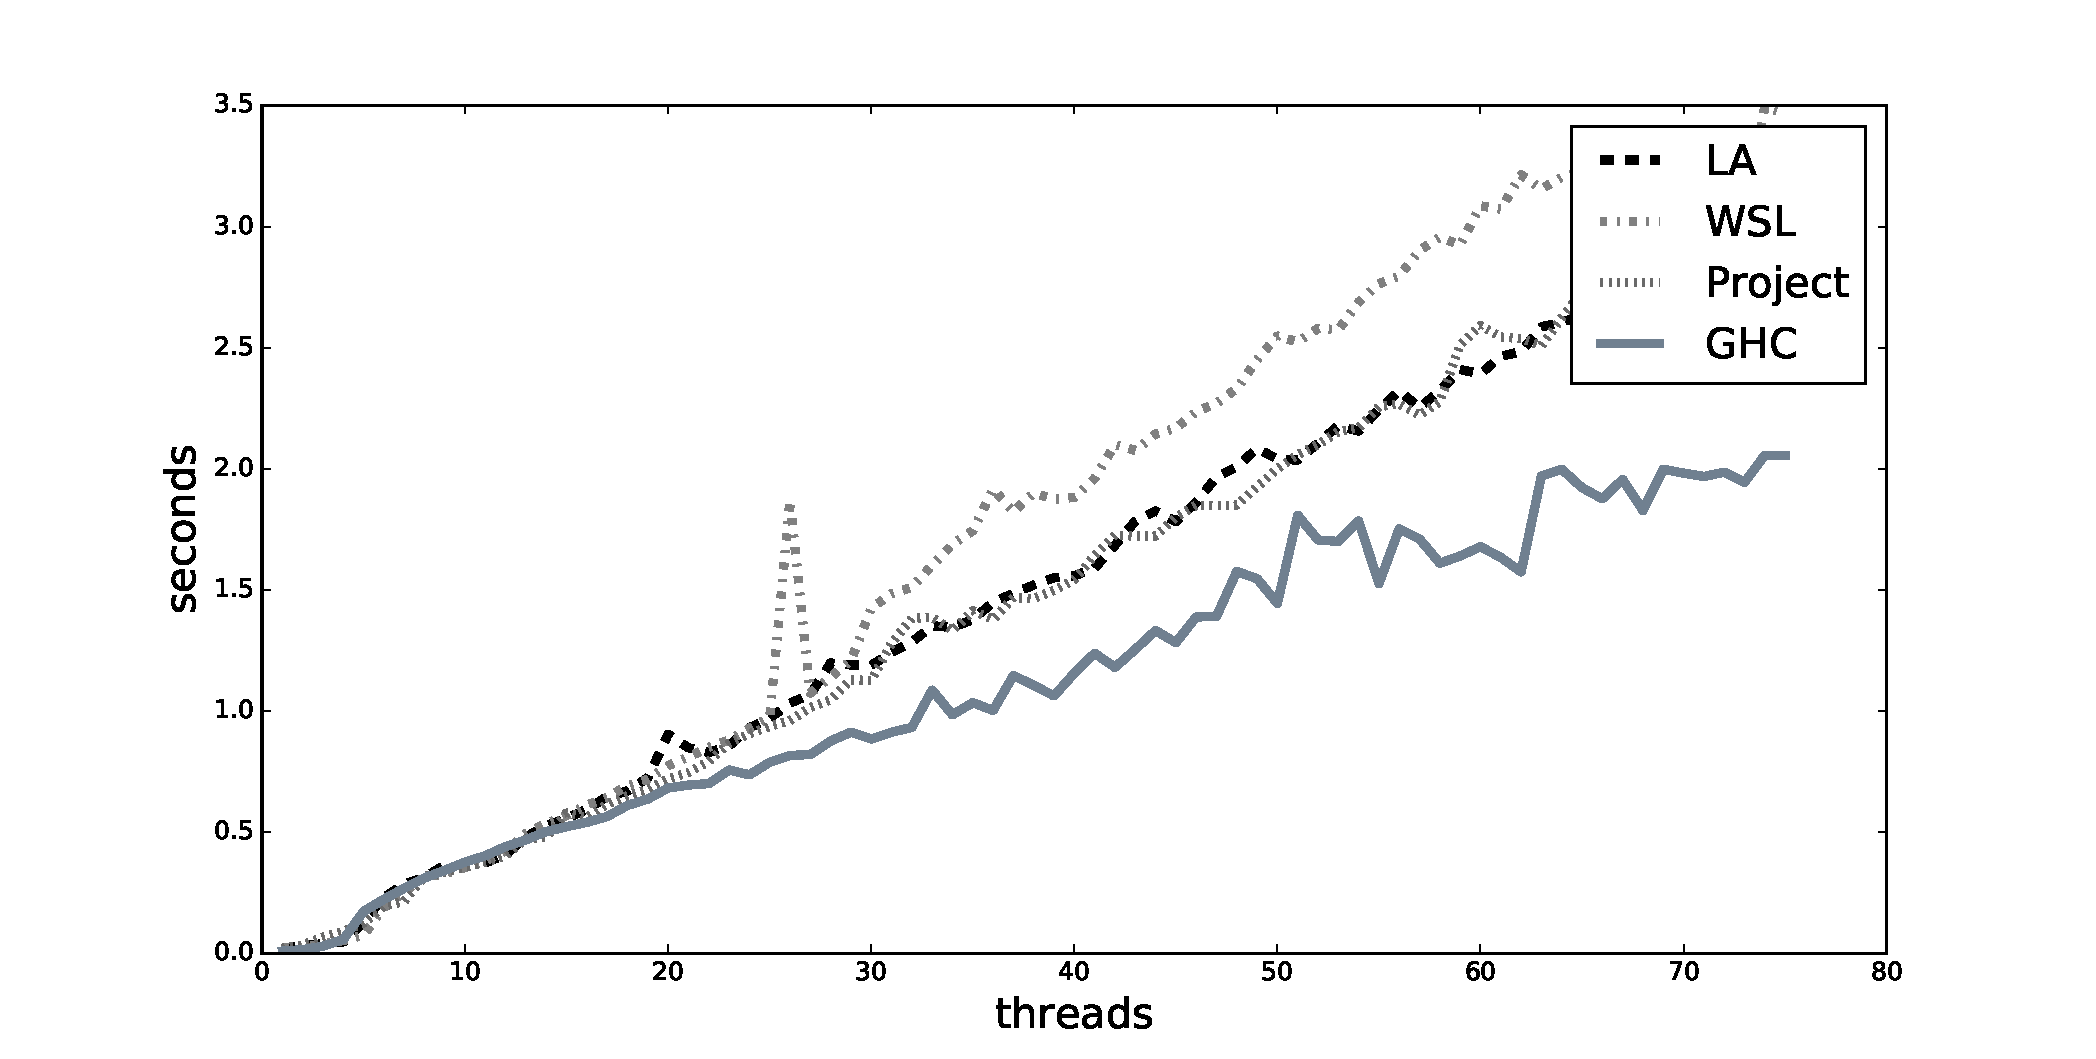
\includegraphics[scale=0.4]{Figures/Scaling1}
\caption[Runtime: Scaling Test I]{Results of the scaling tests with \code{StmTest}}
\label{fig:scaling1}
\end{figure}

Figure \ref{fig:scaling1} show the result of the scaling test performed with \code{StmTest}. We used the following 
configuration: 500 iterations per thread, 100 TVars stored in a list and 20 modifications per transactions with 
a varying number of threads. The x-axis describes the number of threads, while the y-axis contains the total runtime.
Note that an increase in thread results in an increased total work load. The means the increase in runtime in all implementation
is not only due to the fact that the level of concurrency is increased but also due to the increase of the total workload.
All implementations scale equally. The GHC implementation is slightly better and STMWSL is slightly worse than the other 
implementations. Overall, increases the runtime linear with number of threads. The GHC implementation stands out because of
its unstable execution time in this test series. Nevertheless, it still performs better than the other implementations.

\begin{figure}
 \centering
 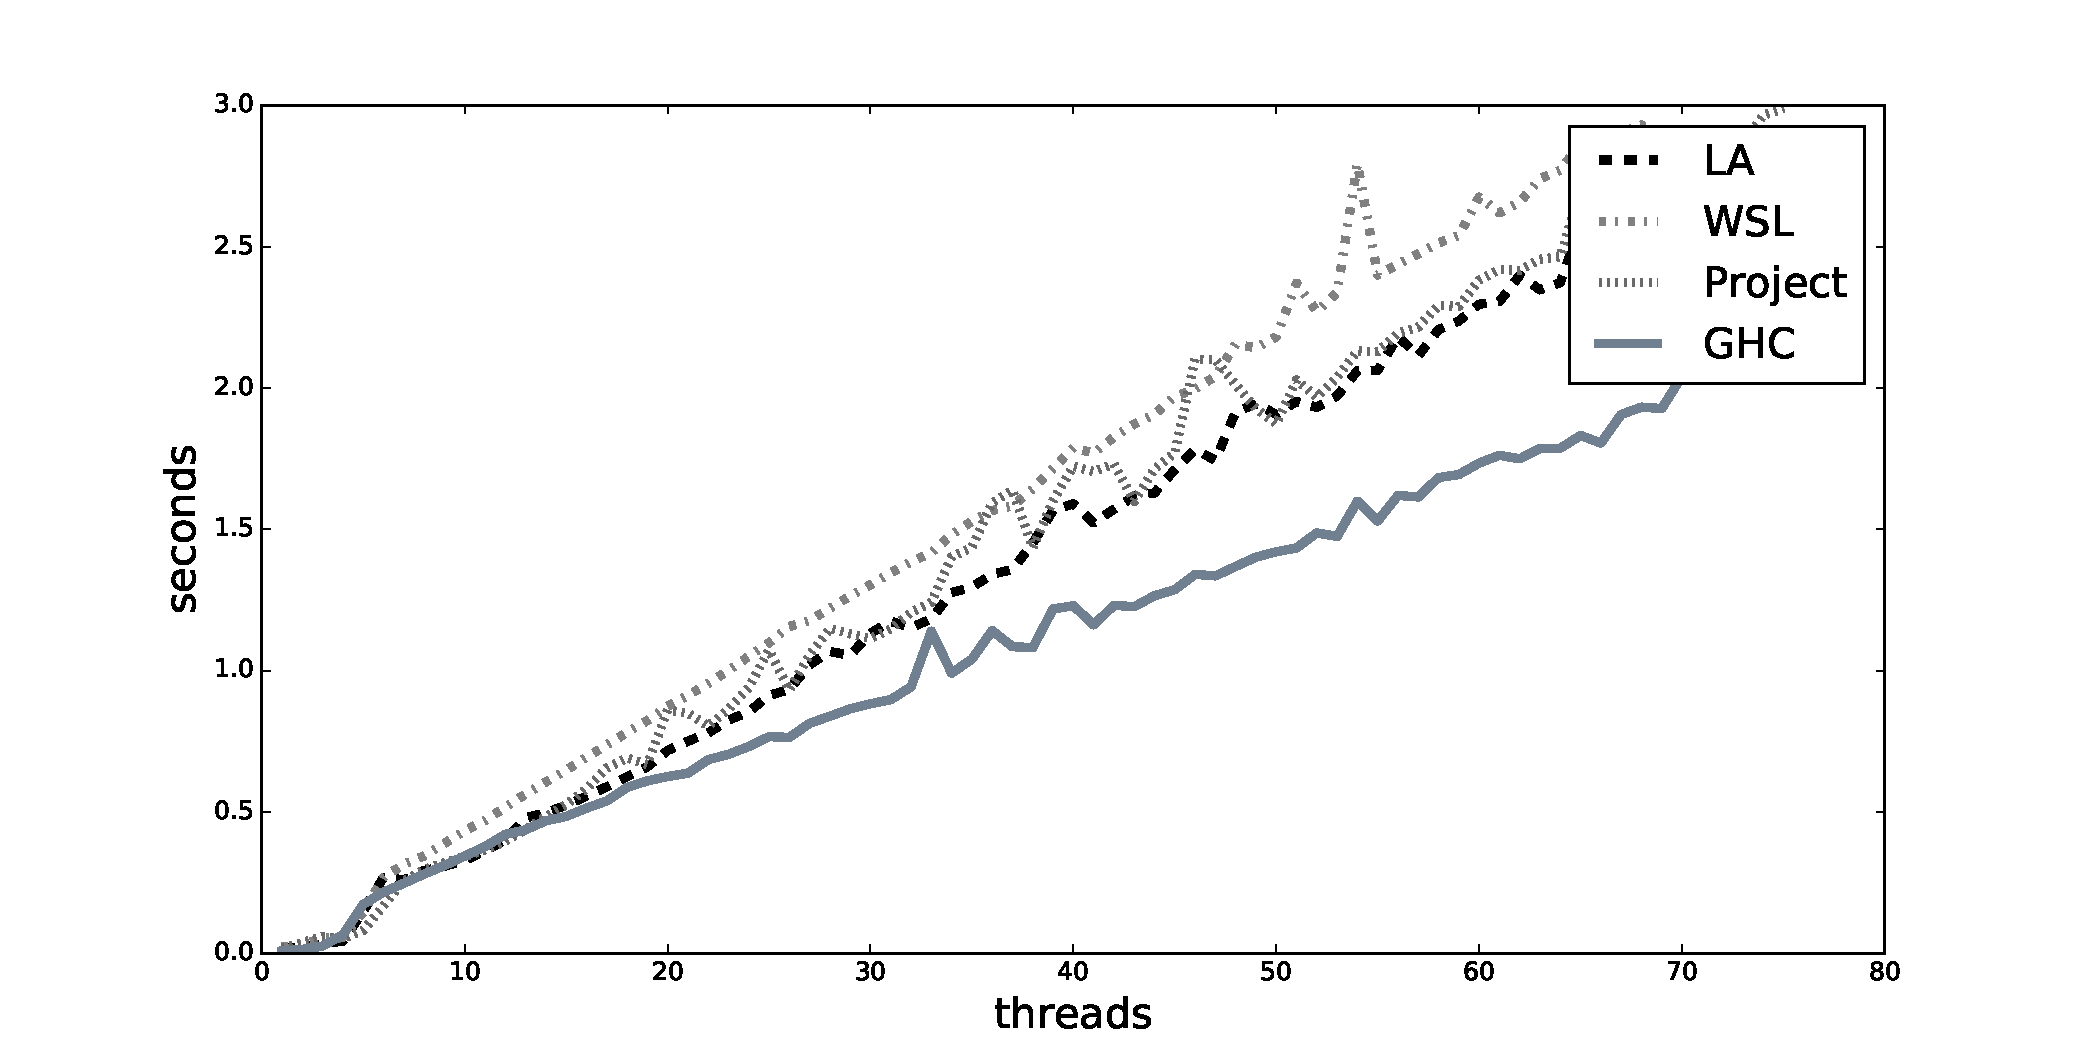
\includegraphics[scale=0.4]{Figures/Scaling2}
\caption[Runtime: Scaling Test II]{Results of the scaling tests with \code{PerformanceTest}}
\label{fig:scaling2}
\end{figure}

The results of the scaling tests performed with \code{PerformanceTest} are presented in Figure \ref{fig:scaling2}. The configuration 
is as follows: 500 transactions per thread, 200 TVar stored in an \code{IntMap}, five times more reads than write and
five writes per transaction (25 read operations per transaction). The results are similar to the previouse results. All implementation scale on equally while
GHC is a slightly faster and STMWSL slightly slower. The differences in the execution time of GHC are less noticable than 
in the first test. The execution time of the project implementation on the other hand varies much more in this test than
in the first test. Nonetheless, the general tendencies are not different. 

This test series show that all implementations are scalable. That GHC performs better than the highlevel implementations
is not surprising. In contrast to the tests presented in the previouse section, these test consist of small transactions.
The GHC implementation uses a very light weighted locking scheme. This makes the commit phase of the GHC implementation
significantly faster than the commit phase of the high level implementation. Thus the fixed (per transaction) overhead
of the highlevel implementations is higher than that of the GHC implementation. Since these tests use smaller transactions
than the first series, the results are reasonable.

\subsection{Observations}
While executing the tests, I noticed that the runtime option \code{N} that creates multiple OS threads slows down the 
computation as a whole. The runtime option \code{N} allows the user to specify the number of OS threads by adding a 
number. I performed some test with runtime options varying \code{N1} to \code{N4} (since the processor contains four 
physical cores). The results are clear. The more OS thread the test uses the slower is the test. This is unpleasant 
because it means our efforts to utilize multi-core processors are futile. To avoid confusion, I am not saying that 
the computation is less efficient; it is slower. For example, one test takes 1.6 second when executed with \code{N1}
and the \textbf{same} test takes 2.3 seconds when executed with \code{N2} (2.6 with \code{N3} and 3.6 with \code{N4}).
The test consumed in the case of \code{N1} a singel core to its full extend (100\%). When the test runs with \code{N2}
it uses two cores, but not to their full extend (around 70\% per core). With \code{N3} it is about 50\% per core and 
with \code{N4} it is about 45\% per core. The system is not utilized by any other process (expect for the OS) while
testing. Even though the total amount of CPU cicles increases with the number of OS threads used, the execution time 
as a whole slows down. I did not take any efforts to explore the reason for this. This is most likely a problem 
in the runtime systems and thus would go beyond the scope of this thesis. The fact remains that in this kind of
setup an increase in OS threads a decrease in performance entails. This \textit{kind of setup} is that most of 
the code is transactional code. A real worlds program is usually not structured like these tests. The portion
of transactional code is far less. Hence this observation does not necessarily mean that STM is useless in 
practise. Nevertheless, all tests presented in this section are executed with \code{N4} to allow real parallelism. 

In addition to the performance test, I performed tests to check the implementations for memory leaks. The GHC implementation
as well as STMLA and STMWSL do not produce memory leaks as far as tested. The Project implementation on the other hand 
contains a memory leak. When ever a transaction reads a TVar, it enters its \code{retryMVar} to the queue of the TVar
to allow other transactions to notify it. If the TVar is never written, but continuously read, this queue grows
and is never emptied. The transactions themself do not remove the MVar from the queue when they rollback or commit.
This is for performance reasons because it requires the transaction to search for its own MVar in all TVar queues it 
has accessed. In STMWSL and STMLA the only time a transaction adds something to the queue is when it executes 
\code{retry}. Additionally removes the transaction its MVar from the queue, when it is not longer needed. In this 
case the performance is not as important as it is for the Project implementation. The \code{retry} either suspends 
the transaction and thus removing the MVars from the queues is a minor performance issue or it does not add the MVar to
the queue at all. The other entries of the TVar can not produce any memory leaks because they can only contain one entry
at a time. Since the log is discarded each time the transaction rolls back or successfully commits, unused data is stored
within the log.